%% -*- coding: utf-8 -*-
\documentclass[12pt,a4paper]{report}
\usepackage[left=2cm,right=2cm,
    top=2cm,bottom=2cm,bindingoffset=0cm]{geometry} 
\usepackage[utf8]{inputenc}
\usepackage[english,russian]{babel}
\usepackage{indentfirst}
\usepackage{misccorr}
\usepackage{graphicx}
\usepackage{amsmath}
\usepackage{amsfonts}
\usepackage{amssymb}
\setcounter{page}{2}
\begin{document}

\begin{titlepage}
\newpage
  \begin{center}
     
    Санкт-Петербургский Политехнический Университет Петра Великого \\
    
    Институт компьютерных наук и технологий \\
    
    Кафедра компьютерных систем и программных технологий
    \end{center}
    
    \vspace{15em}
    \begin{center}
    \textsc{Лабораторная работа №3}\\
    \vspace{5mm}
    \textsc{Линейная фильтрация}
    	
   \end{center}
\vspace{10em}

\newlength{\ML}
\settowidth{\ML}{«\underline{\hspace{0.7cm}}» \underline{\hspace{2cm}}}
\hfill\begin{minipage}{0.45\textwidth}
\vfill
  Руководитель \\
  \\
  \underline{\hspace{\ML}} Богач Н.\,В.\\
 
\end{minipage}%
\bigskip

\hfill\begin{minipage}{0.45\textwidth}
  Выполнил\\
  \\
  \underline{\hspace{\ML}} Солдатова Е.\,И.\\
  группа 33501/3
\end{minipage}%

\vspace{\fill}
\begin{center}
    
  Санкт-Петербург\\
   2018 
\end{center}
\end{titlepage}

\paragraph{1. Цель работы\\\\}
Изучить воздействие ФНЧ на тестовый сигнал с шумом

\paragraph{2. Постановка задачи\\\\}
Сгенерировать гармонический сигнал с шумом и синтезировать ФНЧ. Получить сигнал во временной и частотной областях до и после фильтрации. Сделать выводы о воздействии ФНЧ на спектр сигнала.

\paragraph{3. Теоретическая часть \\\\}
Под фильтрацией электрического сигнала обычно понимают выделение в сигнале желательных спектров, или подавление нежелательных. Тема фильтрации весьма обширна, и рассматривает множество различных подходов к обработке электрического сигнала. Существует масса различных классификаций фильтров, включая:

• аппаратные и программные;

• цифровые и аналоговые;

• линейные и нелинейные;

• фильтры средних, низких и высоких частот;

и т.п.

В данной работе мы рассмотрим один из самых распространенных электронных фильтров — фильтр низких частот (ФНЧ, low pass filter), а точнее — его программную реализацию. Данный тип фильтров используется для сглаживания показаний различных датчиков и сигналов управления.

Резкое усечение импульсной характеристики приводит к сильной изрезанности частотной характеристики в полосе пропускания и недопустимо большому уровню боковых лепестков в полосе непропускания. Чтобы улучшить вид частотной характеристики, импульсную характеристику умножают на весовую функцию (так называемое «временное окно»), которая близка к единице в середине и плавно убывает к краям. В результате форма импульсной характеристики становится более плавной и, как следствие этого, улучшается вид частотной характеристики.

Наилучшие результаты получаются при использовании окна Кайзера, которое описывается выражением:

\begin{figure}[h!]
\center{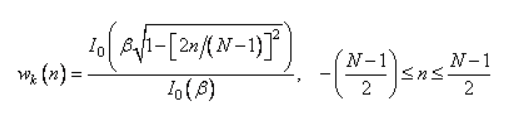
\includegraphics[width=0.5\linewidth]{1}}
\end{figure}

где $\beta$ — константа, определяющая компромисс между максимальным уровнем боковых лепестков и шириной главного лепестка (или долей общей энергии в главном лепестке) частотной характеристики окна.

Окно Кайзера является оптимальным окном в том смысле, что оно представляет последовательность конечной длины, которая имеет минимум энергии спектра за пределами некоторой заданной частоты. 

Однако, ни одно из этих окон не позволяет получить оптимальную в минимаксном смысле аппроксимацию произвольной идеальной частотной характеристики, поскольку в действительности характеристика фильтра является результатом свертки частотных характеристик окна и идеального фильтра. Таким образом, несмотря на наличие оптимальных окон, оптимальных фильтров, которые рассчитывались бы с их помощью, не существует.

\paragraph{4. Ход работы \\\\}

Зададим косинусоидальный сигнал, зашумим его, построим его спектр. Затем используя fdatool создадим фильтр.

Текст программы:\\\\
function Hd = filter\_hd
\%FILTER Returns a discrete-time filter object.\\
\% MATLAB Code\\
\% Generated by MATLAB(R) 9.1 and the DSP System Toolbox 9.3.\\
\% Generated on: 06-Apr-2018 13:10:45\\
\% FIR Window Lowpass filter designed using the FIR1 function.\\
\% All frequency values are in Hz.\\
Fs = 100; \% Sampling Frequency\\\\
N    = 500;      \% Order\\
Fc   = 10;       \% Cutoff Frequency\\
flag = 'scale';  \% Sampling Flag\\
Beta = 0.5;      \% Window Parameter\\\\
\% Create the window vector for the design algorithm.\\
win = kaiser(N+1, Beta);\\\\
\% Calculate the coefficients using the FIR1 function.\\
b  = fir1(N, Fc/(Fs/2), 'low', win, flag);\\
Hd = dfilt.dffir(b);\\\\
\% [EOF]\\\\
t = 0:0.01:4*pi;\\
f0 = 1;\\
x = cos (2*pi*f0*t);\\
figure;\\
plot(t, x); \%исходный сигнал\\\\
x\_noise = awgn (x, 12);\\
figure;\\
plot (t, x\_noise); \%зашумленный сигнал\\\\
figure;\\
plot (t, abs(fft(x\_noise))); \%спектр сигнала\\\\
\%fdatool -> создание фильтра\\
y = filter(Hd, x\_noise);\\
figure;\\
plot (t, y);\\
end\\

Результаты работы в окне fdatool для различных параметров:

\begin{figure}[h!]
\center{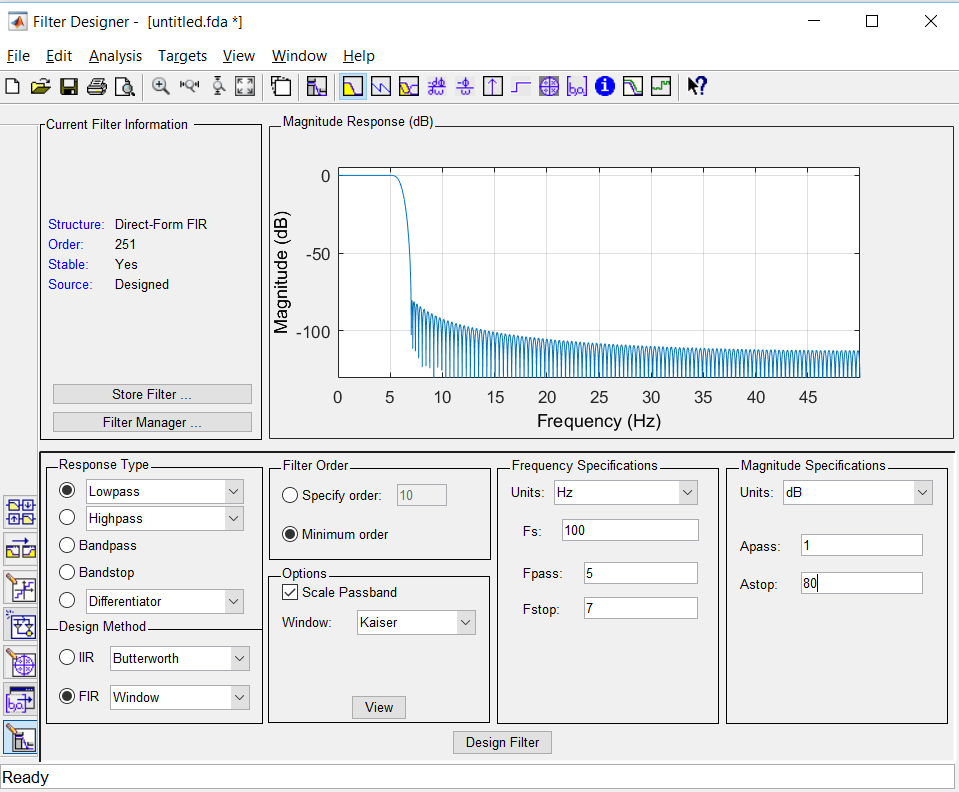
\includegraphics[width=0.5\linewidth]{Filter}}
\end{figure}

\begin{figure}[h!]
\center{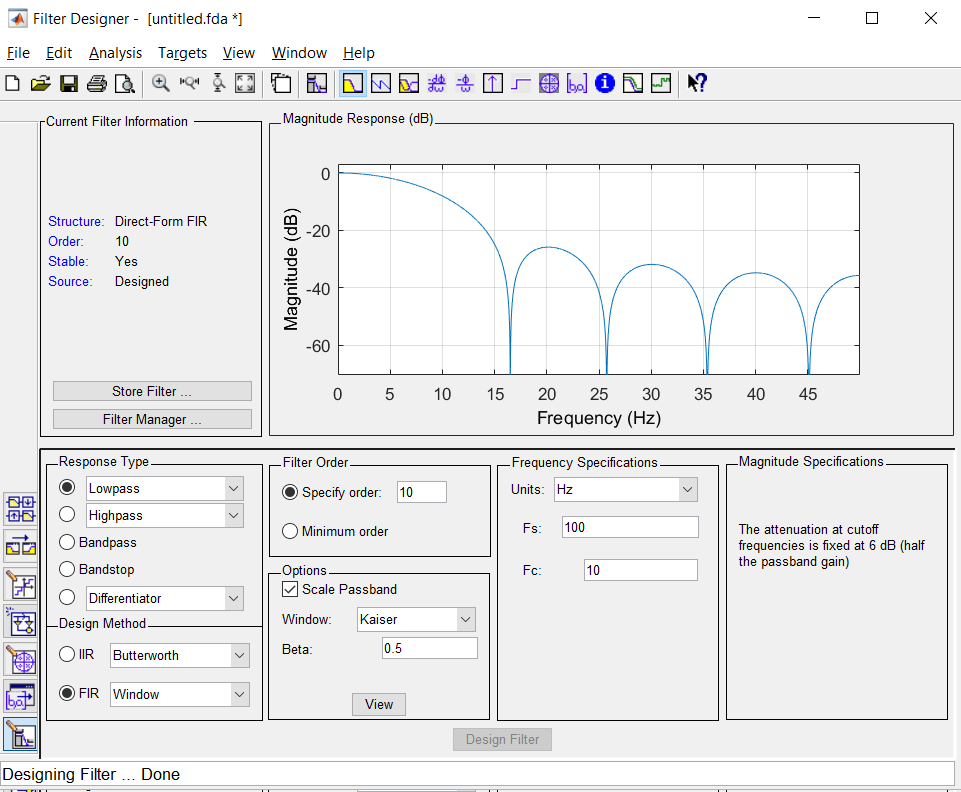
\includegraphics[width=0.5\linewidth]{Filter-1}}
\end{figure}

\begin{figure}[h!]
\center{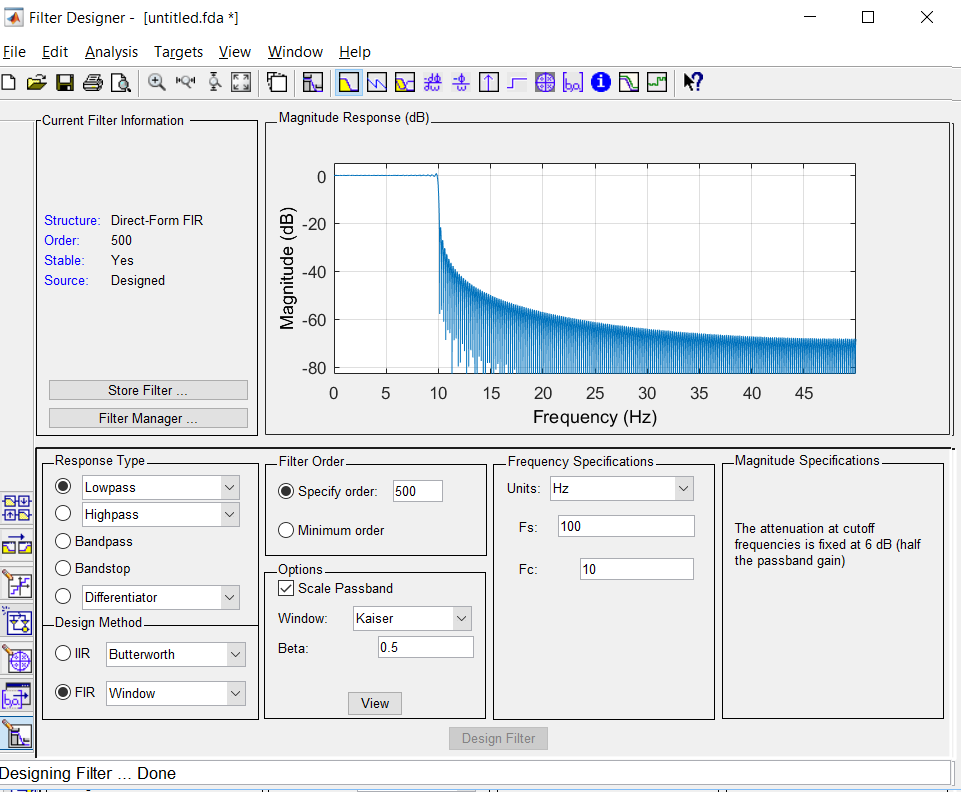
\includegraphics[width=0.5\linewidth]{Filter-3}}
\end{figure}

\paragraph{5. Выводы\\\\}

Итак, используя фильтр, мы  устраняем большую часть помех и тем самым улучшаем качество сигнала. Однако часть шума может совпадать с сигналом, и фильтр не сможет его убрать. Для получения лучших результатов используются окна, и одно из самых известных - это окно Кайзера.

При увеличении $\beta$ в окне Кайзера уменьшается уровень боковых лепестков частотной характеристики и пульсации в полосе пропускания и в то же время уменьшается крутизна скатов частотной характеристики. С помощью окна Кайзера можно синтезировать фильтры, имеющие практически прямоугольную форму частотной характеристики.
\end{document}